\RequirePackage[T1]{fontenc}
\documentclass[journal,onecolumn]{IEEEtran}
\usepackage{amsmath,amssymb,bm,graphicx}
\begin{document}
\title{Supplementary Method Diagrams}
\author{Hongyu~Chen, Peng~Liu,~\IEEEmembership{Senior~Member,~IEEE,}
and~Yaqiu~Jin,~\IEEEmembership{Life~Fellow,~IEEE}}
\maketitle
\noindent\textbf{Accompanying article:} SAR Despeckling via Fourier Refinement and Representation-Consistent Reconstruction.
\par\smallskip
\noindent\emph{Corresponding author: Peng Liu.}
\par\smallskip
\noindent The authors are with the Key Laboratory of Information Science of Electromagnetic Waves, Fudan University, Shanghai, China (e-mail: \mbox{pliu@fudan.edu.cn}).
\par\medskip
\noindent These diagrams illustrate the refinement, reconstruction, and adaptation operations fully specified in Section~II of the main article. They provide no additional experiments or results. All experimental tables and comparison figures appear in the five-page main manuscript.
\par\bigskip
\noindent
\begin{minipage}[t]{0.48\textwidth}
\centering
\vspace{0pt}
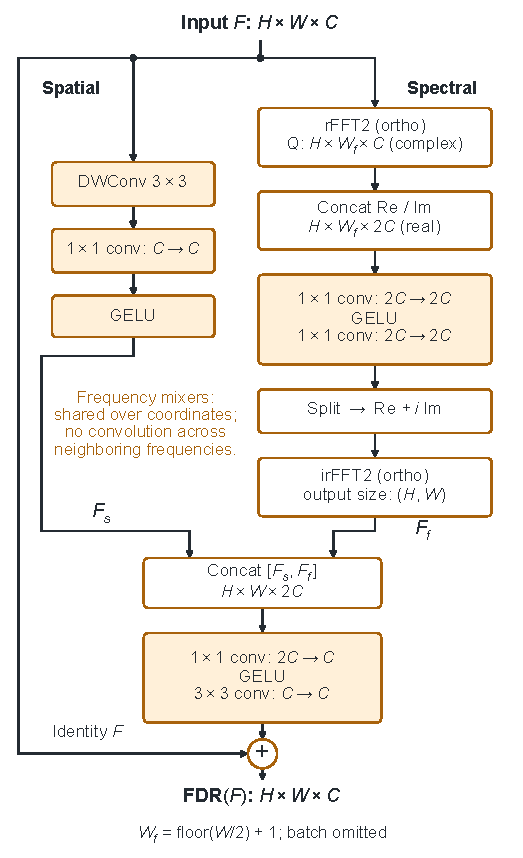
\includegraphics[width=0.94\linewidth,trim=0 5bp 0 6bp,clip]{figures/fig2_fdr_block.pdf}\par\medskip
{\footnotesize\raggedright\textbf{Fig. S1.} Full-spectrum Fourier residual refinement (FDR). Local depthwise--pointwise filtering runs in parallel with spectral refinement. The one-sided rFFT contains all nonredundant frequencies. Real-valued \(1\times1\) convolutions share weights across frequency coordinates and mix the real and imaginary channels at each coordinate. An inverse rFFT restores spatial features, which are concatenated with the local features, projected, and added to the input.\par}
\end{minipage}\hfill
\begin{minipage}[t]{0.48\textwidth}
\centering
\vspace{0pt}
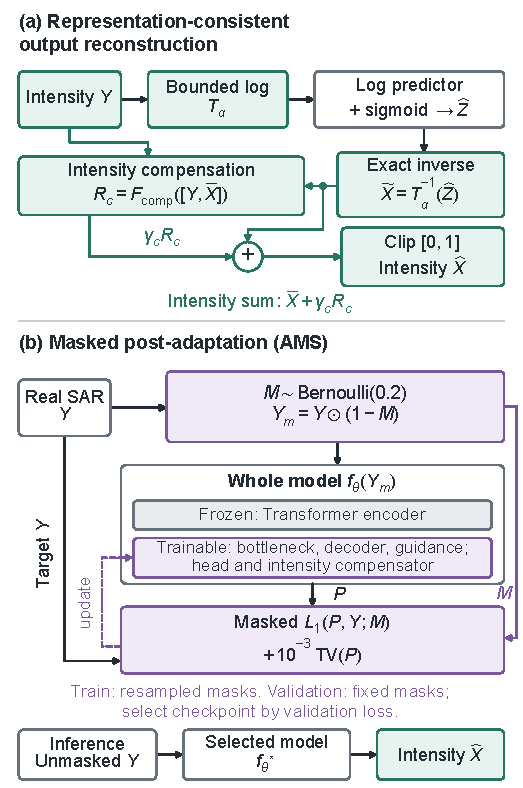
\includegraphics[width=0.98\linewidth,trim=0 2bp 0 5bp,clip]{figures/fig3_representation_ams.pdf}\par\medskip
{\footnotesize\raggedright\textbf{Fig. S2.} (a) Reconstruction applies exact inversion before intensity residual
  compensation and clipping. (b) In AMS, the complete network, including the
  compensator, receives $Y_m$ in place of the generic input $Y$ in (a);
  unmasked $Y$ provides the noisy target. The Transformer encoder alone is
  frozen. Resampled training masks drive adaptation, fixed validation masks
  guide checkpoint selection, and inference uses unmasked observations.\par}
\end{minipage}
\end{document}
